\documentclass{standalone}
\usepackage{standalone}

\begin{document}

\subsection{Converting to Binary Image}
The image from previous stage is need to be converted in binary for convenience. Bangladeshi license plates have two types: white text on black plate for private cars and black text on white plate for public ones. To be accurate, we first converted the image into black and white using two filters: $THRESH_BINARY$ one time and $THRESH_BINARY_INV$ the other. Then compared the ratio of non-zero pixels of each image. The image which has lesser ratio, most probably is selected as the expected binary image. 

Figure \ref{fig:BlackAndWhite} shows the conversion to binary images using the above algorithm for different types of license plates.

\begin{figure}
\begin{subfigure}{.5\textwidth}
  \centering
  
\includegraphics[width=.8\linewidth]{./img/sample/bnw-1.jpg}
  \caption{A private license plate}
  \label{fig:PrivatePlate}
\end{subfigure}
\begin{subfigure}{.5\textwidth}
  \centering
  
\includegraphics[width=.8\linewidth]{./img/sample/bnw-2.jpg}
  \caption{Black and white image of \ref{fig:PrivatePlate}}
\end{subfigure}
\begin{subfigure}{.5\textwidth}
  \centering
  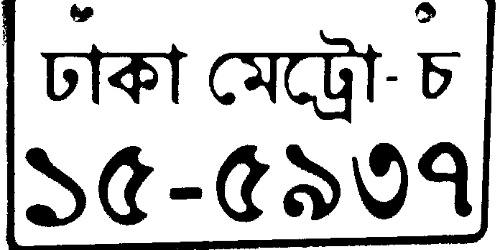
\includegraphics[width=.8\linewidth]{./img/sample/bnw-3.jpg}
  \caption{A public license plate}
  \label{fig:PublicPlate}
\end{subfigure}
\begin{subfigure}{.5\textwidth}
  \centering
  
\includegraphics[width=.8\linewidth]{./img/sample/bnw-4.jpg}
  \caption{Black and white image of \ref{fig:PublicPlate}}
\end{subfigure}
\caption{Black and white conversion of two types of image}
\label{fig:BlackAndWhite}
\end{figure}


\end{document}